\documentclass[12pt]{article}
\usepackage[utf8]{inputenc}
\usepackage[english]{babel}
\usepackage[table,xcdraw]{xcolor}
\usepackage{hyperref}
\usepackage{float}
\usepackage{amsmath}
\usepackage{mathtools}
\usepackage{tikz}
\usepackage{pgfplots}


\pgfplotsset{compat=1.14}

W
\hypersetup{
	colorlinks,
	citecolor=black,
	filecolor=black,
	linkcolor=black,
	urlcolor=black
}

\usepackage[backend=biber,style=authoryear]{biblatex}
\usepackage[newfloat]{minted}
\usepackage{csquotes}
\usepackage{caption}


\graphicspath{ {images/} }


\usemintedstyle{vs}

\newcommand\tab[1][1cm]{\hspace*{#1}}
\SetupFloatingEnvironment{listing}{name=Code example}
\definecolor{bg}{rgb}{0.95,0.95,0.95}
\newenvironment{code}{\captionsetup{type=listing}}{}

\newcommand\codeblock[3]{%
\begin{code}
	\caption{#3}
	\inputminted[%
	    mathescape,
	    linenos,
	    numbersep=5pt,
	    tabsize=4,
	    label=Helloworld,
	    bgcolor=bg,
	    breaklines%
	]{TypeScript}{#1}
	\label{#2}
\end{code}
}

\newcommand\Code[1]{\texttt{#1}}

\addbibresource{sample.bib}

\begin{document}

\begin{titlepage}
	\centering
	\vspace{2cm}
	{\Huge Analysis of voting systems: What should I call it? \par}
	\vspace{0.6cm}
	{\LARGE Adrian Salamon\par}

	\vspace{0.6cm}
	{\Large Kungsholmens gymnasium\par}
	\vspace{0.4cm}
	{\large Senior thesis\par}
	\vspace{0.6cm}
	
\includegraphics[width=0.3\textwidth]{kg}\par\vspace{1cm}
	\vspace{4cm}
	\vfill
	Supervised by: \par
	Maja Kankaanranta

	\vfill

	% Bottom of the page
	{\large \today\par}
\end{titlepage}

\pagebreak

\begin{abstract}
	The abstract text goes here.
\end{abstract}

\pagebreak

\tableofcontents

\pagebreak

\section{Introduction}
\subsection{Background}
Taking a collective decision as a population is difficult. To solve this issue, voting systems with defined rules are used. They are used to show common preferences within a population, for example what politician a population wants to see elected. Several types of systems have been designed and there are a myriad of variations of those systems. They range from simple methods such as “most votes win” to complex processes that can only be practically carried out by a computer. However, practically all voting systems are algorithmic in nature, which makes them interesting to study for both Computer Scientists and Mathematicians. When deciding on what systems that shall be used, it is useful to know what differences and similarities they have.
\subsection{Purpouse}
The purpose of this essay is to evaluate differences and similarities in terms of election results in three different voting systems: Single Transferable Vote (STV), First-Past-The-Post (FPTP) and the Schulze Method. This paper will only be examining and discussing differences and similarities in the results of the methods, not touching on how practically feasible the methods might be in actual election.
\pagebreak
\section{Theory}
Theory will be here some day
\section{Methodology}
All voting methods have been implemented in Typescript – mostly due to the author having previous experience with JavaScript. Typescript is a superset of JavaScript with multiple extra feautures. Most importantly Typescript has optional static type checking. Here is some example code in typescript:
\codeblock{code/typescriptexample.ts}{code:typescript example}{Basic Typescript syntax}
\subsection{Modeling test data}
In order to test the methods and their implementations, test data is needed. There are cases where extensive election data is published, such as in maltese elections, but full ballot data, which is needed for the implementations has not been found. Instead, the implementations will be tested with data generated from a simple computer algorithm. The algorithm used in this paper is highly primitive, as modeling prefrences within a population is far beyond this paper. The full ballot generation program can be found in the \Code{/generator/} folder. The goal of the program is to produce ballots that rank every candidate in order of prefrence (see figure \ref{STV ballot} on page \pageref{STV ballot}). The program represents each voter in a population as belonging to a certain ideology. Each ideology has has a list of weighted prefrences indicating how a voter for this ideology is likely to vote. The weighed prefrences are generated via an abstraction. A single config object is used to create all ideologies.
\codeblock{code/generator/ideologyConfig.ts}{code:ideology config}{Configuration object for creating ideologies}
The program then works via 4 major steps:
\begin{enumerate}
	\item It relates each candidate to an ideology based on the size of the ideology. A larger ideology has more candidates.
	\item It assigns a base size for each candidate. Each ideology has a different spread of votes generated by a negative exponential function with a different constant. The size of each candidate is then multiplied with the size of their ideology and normalized. This gives a base size of all candidates.
	\item Based on the base size of each candidate, a probability-list of voting for each candidate is created for every ideology. An ideology's probability-list represents how a voter aligned the ideology is expected to vote.
	\item It creates a certain number of individual ballots. Each ballot is given an ideology and creates its own list prefrences based via weighted random number generaton according to the probability-list of the assigned ideology.
\end{enumerate}
The output of the program is a set of ballots, where each ballot is an ordered set of prefrences. The implementation is highly arbitrary and all constants in the program even more so. However, expanding on the generator program would be beyond the scope of this project. The program works in that it is possible to control variables to test for different election scenarios.
\subsection{Constructing test scenarios}
Constructing test scenarios is difficult task. Due to there being so many variables both in real elections and the simulated elections in the generator program, it makes it practically inpossible to control all variables. Instead, 3 arbitrary test scenarios will be used. The election will be simulated 1000 times for each scenario and the election data will then run through the different voting methods and the results will be compared. The simulation scenarios are arbitrary but should allow for comparison of the different voting methods. All simulations will have 3 ideologies and 500 voters.
\subsubsection{Scenario 1}
Scenario 1 is this:
\codeblock{code/generator/scenario1.ts}{code:scenario 1}{Scenario 1}


\pagebreak
\section{Specification of voting methods}
This paper compares the results of theese voting methods
\subsection{First-past-the-post}
\subsubsection{Description}
The first-past-the-post voting method is a method desiged for electing one or several candidates out of a set of candidates. Each voter has one (1) vote which may be allocated to any candidate. In a first-past-the-post election the N candidates with most votes get elected.
\subsubsection{Justification}
The method is simple and can easily be understood. The first-past-the-post method is widely used in for example the United Kingdom and United States. Comparisons with this method can also be easily made.
\subsubsection{Pseudocode}
let $V$ be the set of votes with $V_{i}$ being the number of votes for candidate $i$ \\
let $N$ be number of candidates to be elected \\
sort $V$ based on $V_{i}$\\
slice $V$ between $0$ and $N$
\subsubsection{Implementation}
The first-past-the-post program is implemented in a single file. It takes the following inputs:
\codeblock{code/fptp/inputs.ts}{code:fptp inputs}{Inputs for FPTP program}
The ballot data is first mapped to only include first prefrences. Then the algorithm loops over the ballots and gets the sum of votes for each candidate:
\codeblock{code/fptp/processing.ts}{code:fptp processing}{Processing and formatting of data}
The results array is sorted and sliced to only include the $N$ candidates with most votes:
\codeblock{code/fptp/result.ts}{code:fptp result calculation}{Finding and returning winning candidates}
\subsection{Single transferable vote}
\subsubsection{Description}
The Single Transferable Vote method is a more complicated algorithm than the first-past-the-post method. Voters are given ballots where they are supposed to rank candidates in order. The specific rules for if you need to rank all candidates or rank several candidates at the same value not can vary. For the sake of simplicity, in this implementation, all candidates must be ranked at unique and linear values. A ballot may look like this:
\begin{figure}[H]
	\centering
	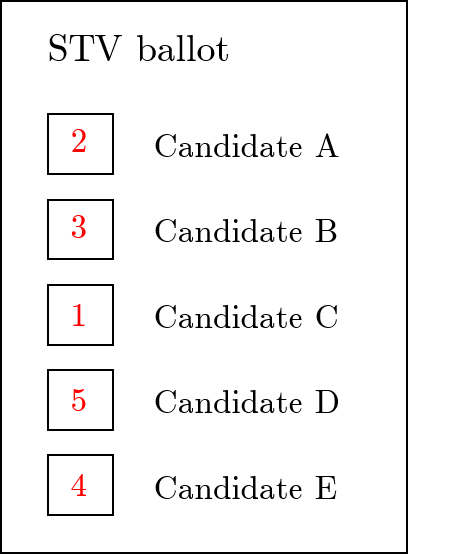
\includegraphics[height=140px]{ballot}
	\caption{Sample STV ballot}
	\label{STV ballot}
\end{figure}
This means that there is more data availible for detrermining the result of the election which the method can take advantage of. Votes are, if needed, transfered between choices within a ballot, hence the name Single Transferable Vote. The method relies on the concept of a quota, the number of votes you need to be elected. The Droop-Quota, defined as $(\frac{\text{total valid poll}}{\text{seats} + 1})+1$, is often used. If a candidate recieves equal or more votes than the quota, he/she is elected. If the number of votes exxeed the quota, a fraction of the votes are transfered to the next choice on the ballots that voted for the elected candidate. This process is repeated until there are no candidates with more votes than the quota. If there still are seats yet to be filled, the candidate with fewest votes is eliminated and his/her votes are transfered to the next choice on those ballots. This process is repeated until all seats are filled. The process can become quite complex with many ballots and transfering fractional votes. In order to resolve large scale elections, a computer in essential.
\subsubsection{Justification}
STV is an established voting method in use in several countries. It is used for parlimentary elections in Ireland, Malta and Australia as well as being used in local and regional elections across the world.
\subsubsection{Pseudocode}
\label{Stv psuedocode}
let $quota$ be the quota \\
let $seats$ be the number of seats \\
let $winners$ be the list of elected candidates \\
let $votes$ be the set of votes with $votes_{i}$ signinfying votes for candidate $i$\\
while $\left\vert{winners}\right\vert < seats$\\
\tab if any candidate $i \notin winners$ and $votes_{i} \geq quota$ \\
\tab\tab add $i$ to $winners$ \\
\tab\tab continue \\
\tab end if \\
\tab if any candidate $i$ where $votes_{i} > quota$\\
\tab\tab multiply $votes_{i}$ with $(1 - \frac{\text{surplus votes}_{i}}{votes_{i}})$ \\
\tab\tab multiply next prefrencences for $votes_{i}$ with $\frac{\text{surplus votes}_{i}}{votes_{i}}$ and \\ \tab\tab distribute into $votes$\\
\tab\tab continue \\
\tab end if \\
\tab if $\left\vert{votes}\right\vert = seats$ \\
\tab\tab add all $votes \notin winners$ to $winners$ \\
\tab\tab continue \\
\tab end if \\
\tab $k \coloneqq$ index of smallest $votes_{i}$ \\
\tab eliminate $votes_{k}$ and distribute all next-prefrence votes for candidate $k$ \tab into $votes$\\
end while
\subsubsection{Implementation}
The single transferable vote algorithm uses a tree structure to represent the state of the election. Every candidate is a top-level node with an attribute showing the number of current votes for the candidate. Each node has child nodes representing the next prefrences of the voters for that particular candidate, see figure \ref{Tree structure}. It is easy to manipulate branches via recursion. Merging and multiplying branches is used when transfering votes from one candidate node to another. A candidate node is a Typescript class. It can be found in the \Code{stv/candidate.ts} file and has the following properties and functions:
\begin{figure}
	\centering
	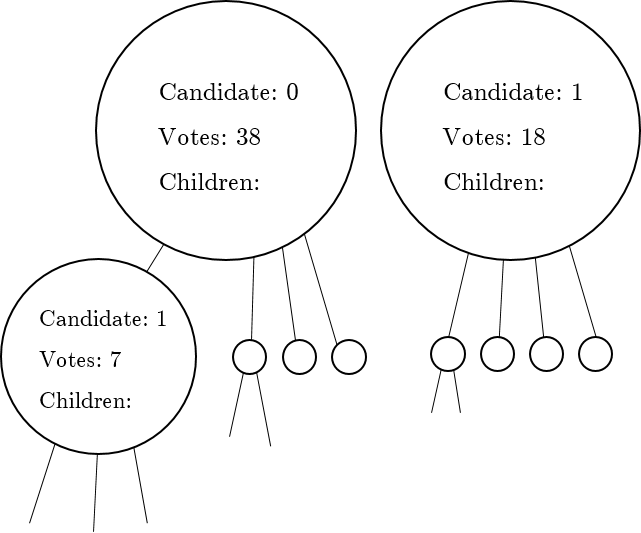
\includegraphics[height=200px]{Tree}
	\caption{Simplified and shortened version of the tree structure. Each candidate is a top-level node with children, signifying the prefrences of the voters for that candidate.}
	\label{Tree structure}
\end{figure}
\codeblock{code/stv/candidateNode.ts}{code:stv candidate node}{The CandidateNode class}
With the \Code{add()} and \Code{multiply()} functions it is possible to recursively modify branches. There are two different manipulations that need to be preformed on the tree: tansfering surplus votes and eliminating candidates. Both functions rely on the \Code{distribute()} function wich is used to distribute a set of nodes onto the tree.
\codeblock{code/stv/distribute.ts}{code:stv distribute function}{The distribute function}
In order to eliminate and transfer surplus votes from any candidate node $A$, the children of $A$ are passed into the distribute function. In the case of transfering surplus votes, the votes for each child node is first multiplied by $\frac{\text{surplus votes}}{\text{total votes}}$ as outlined in the psuedocode in section \ref{Stv psuedocode}. The full source code for funcions that manipulate the tree structure can be found in \Code{/stv/tree.ts}.

The main procces of the program is found in the \Code{stv/election.ts} file and runs the process defined in the psuedocode in section \ref{Stv psuedocode} on page \pageref{Stv psuedocode}.

\subsection{Schulze}
\subsubsection{Description}
The Schulze Method is a method used mainly to determine results in a single-winner election but can also be used to provide rankings and elect multiple candidates in a single election. Ballots are identical to those of the single transferable vote, see figure \ref{STV ballot} on page \pageref{STV ballot}. The method is compliant with the Condorcet Criterion, which means that if there is a candidate who the majority prefers in a pairwise comparison with every other candidate, that candidate wins. As mentioned, this method relies on comparing the prefrences of every candidate to one another as shown in table \ref{Pairwise comparison matrix}. If there is a condorcet winner the process is simple: declare the condorcet winner a winner and run another iteration without that candidate. Repeat this process until all seats are filled. However, there can be condorcet ties, where there is no condorcet winner. There are multiple ways of resolving the tie, one of them being the Schulze Method.

The Schulze Method resolves ties by investigating possible paths between candidates. For example, if out of a total of 50 ballots 30 ballots prefer $B>A$, 28 ballots prefer $A>C$ and 27 ballots prefer $C>B$, a path from $A$ to $B$ can be created by going $A \rightarrow C \rightarrow B$. The path is said to have the $strength$ of the weakest link in the path. In this example, the path strenght between A and B is 27 due to the link between $C$ and $B$ having a strenght of 27. There may be several paths between two candidates and the goal of the process is to find the strongest path between any candidate $A$ and $B$, written as $p[A,B]$. By finding the strongest path between all nodes a result can be obtained where $p[X,Y] \geq p[Y,X]$ wich means that candidate $X$ wins. The Shulze Method also provides a linear ranking between all candidates, for example that $E > B > A > C > D$. By selecting the $N$ top candidates you can use the method for a multi-seat election. As the process can become very complex as the number of candidates grow, a computer is needed to resolve large elections.

The difficult problem in this method is finding the strongest path between candidates. The problem is called the widest path problem in graph theory. An efficent and relatively simple way to compute this problem is via the Floyd-Warshall algorithm which is used in the implementation. See \ref{Schulze psuedocode} for the full algorithm.

\begin{table}[H]
\centering
\begin{tabular}{l|c|c|c|c|c|}
\cline{2-6}
 & \multicolumn{1}{l|}{A} & \multicolumn{1}{l|}{B} & \multicolumn{1}{l|}{C} & \multicolumn{1}{l|}{D} & \multicolumn{1}{l|}{E} \\ \hline
\multicolumn{1}{|l|}{A} & \cellcolor[HTML]{9B9B9B} & \cellcolor[HTML]{FFDDDD}17 & \cellcolor[HTML]{FFDDDD}14 & \cellcolor[HTML]{DDFFDD}35 & \cellcolor[HTML]{DDFFDD}30 \\ \hline
\multicolumn{1}{|l|}{B} & \cellcolor[HTML]{DDFFDD}33 & \cellcolor[HTML]{9B9B9B} & \cellcolor[HTML]{FFDDDD}24 & \cellcolor[HTML]{DDFFDD}47 & \cellcolor[HTML]{DDFFDD}36 \\ \hline
\multicolumn{1}{|l|}{C} & \cellcolor[HTML]{DDFFDD}36 & \cellcolor[HTML]{DDFFDD}26 & \cellcolor[HTML]{9B9B9B} & \cellcolor[HTML]{DDFFDD}40 & \cellcolor[HTML]{DDFFDD}42 \\ \hline
\multicolumn{1}{|l|}{D} & \cellcolor[HTML]{FFDDDD}15 & \cellcolor[HTML]{FFDDDD}3 & \cellcolor[HTML]{FFDDDD}10 & \cellcolor[HTML]{9B9B9B} & \cellcolor[HTML]{FFDDDD}18 \\ \hline
\multicolumn{1}{|l|}{E} & \cellcolor[HTML]{FFDDDD}20 & \cellcolor[HTML]{FFDDDD}14 & \cellcolor[HTML]{FFDDDD}8 & \cellcolor[HTML]{DDFFDD}32 & \cellcolor[HTML]{9B9B9B} \\ \hline
\end{tabular}
\caption{Pairwise comparison matrix used in the Schulze Mehtod. For example, 17 ballots prefer $A>B$ and 33 ballots prefer $B>A$.}
\label{Pairwise comparison matrix}
\end{table}
\subsubsection{Justification}
The Shulze Method is used by multiple organisations around the world. It has been used by various software organisations such as The Wikimedia Foundation, The Debian Project and Ubuntu. It is also used by political parties such as the Pirate Party in Sweden and various other countries. The process also differs greatly in both method and implementation from the two other voting methods used in this paper.
\subsubsection{Pseudocode}
\label{Schulze psuedocode}
let $d[i,j]$ be the number of ballots that prefer candidate $i$ to candidate $j$\\
let $p[i,j]$ be the strength of the strongest path from candidate $i$ to candidate $j$\\
for $i$ from 1 to $C$\\
\tab for $j$ form 1 to $C$\\
\tab\tab if ($i \ne j$)\\
\tab\tab\tab if ($d[i,j] > d[j,i]$)\\
\tab\tab\tab\tab $p[i,j] \coloneqq d[i,j]$\\
\tab\tab\tab else\\
\tab\tab\tab\tab $p[i,j] \coloneqq 0$\\
\tab\tab\tab endif \\
\tab\tab endif \\
\tab endfor \\
endfor\\
for $i$ from 1 to $C$\\
\tab for $j$ form 1 to $C$\\
\tab\tab if ($i \ne j$)\\
\tab\tab\tab for $k$ from 1 to $C$\\
\tab\tab\tab\tab if ($i \ne k \text{ and } j \ne k$)\\
\tab\tab\tab\tab\tab $p[j,k] \coloneqq \text{max }(p[j,k], \text{ min }(p[j,k], p[i,k]))$\\
\tab\tab\tab\tab endif \\
\tab\tab\tab endfor \\
\tab\tab endif \\
\tab endfor \\
endfor\\
\subsubsection{Implementation}
The Shulze Method is implemented within the file \Code{schulze/index.ts}. It takes two inputs: a list of ballots and the number of seats to be elected. A ballot is an ordered list of candidates. The output of the program is a list of winners. The program first creates the matrices for both the prefrences and paths between candidates.
\codeblock{code/schulze/maps.ts}{code:schulze maps}{Data representation}
The program then runs the algorithm outlined in the psuedocode in section \ref{Schulze psuedocode}.
\codeblock{code/schulze/algorithm.ts}{code:schulze algorithm}{Main algorithm}
\section{Evaluation of methods}
\subsection{Sample I}
\subsection{Sample II}
\subsection{Sample III}


\section{Conclusion}





%\subsection{ Heading Here}
%This is some code.
%\lstinputlisting[language=JavaScript]{code/examples/example.js}



%\section{Conclusion}
%Write your conclusion here. And here is a citation:
%\textcite{sigfridsson2}

%And another one here (\textcite{sigfridsson})

%\section{Source code}
%\lstinputlisting[language=JavaScript]{code/test.js}

\pagebreak




\begin{figure}
	\centering
	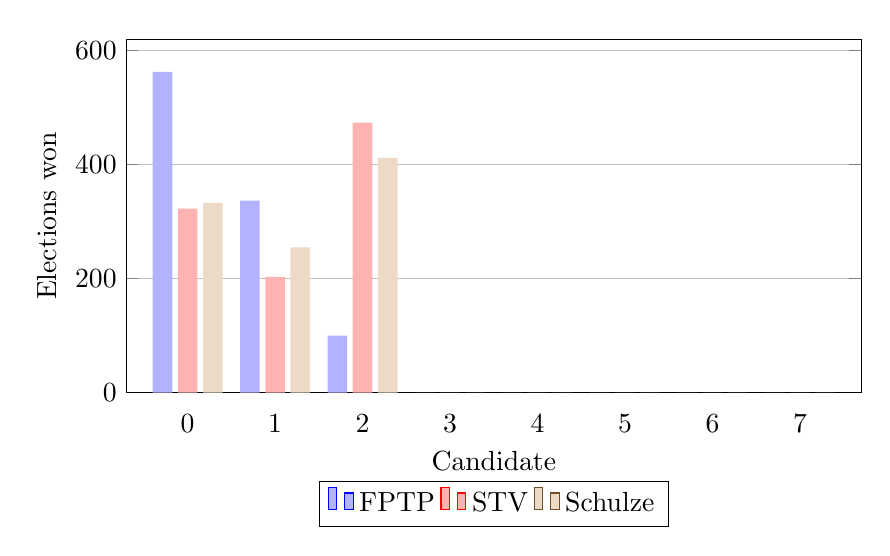
\begin{tikzpicture}
		\begin{axis}[
			ybar,
			width = 0.9\textwidth,
			height = 0.5\textwidth,
			legend style={at={(0.5,-0.25)},
			anchor=north,legend columns=-1},
      x tick style = transparent,
			ylabel = {Elections won},
			xlabel = {Candidate},
			ymajorgrids = true,
			every axis plot/.append style={draw=none,fill,no markers},
      ymin = 0,
			symbolic x coords={0,1,2,3,4,5,6,7,8},
			bar width=0.25cm
      ]
			\addplot coordinates
{(0, 563)(1, 337)(2, 100)(3, 0)(4, 0)(5, 0)(6, 0)(7, 0)};
\addplot coordinates
{(0, 323)(1, 203)(2, 474)(3, 0)(4, 0)(5, 0)(6, 0)(7, 0)};
\addplot coordinates
{(0, 333)(1, 255)(2, 412)(3, 0)(4, 0)(5, 0)(6, 0)(7, 0)};

			\legend{FPTP, STV, Schulze}
		\end{axis}
	\end{tikzpicture}
\end{figure}

\begin{figure}
	\centering
	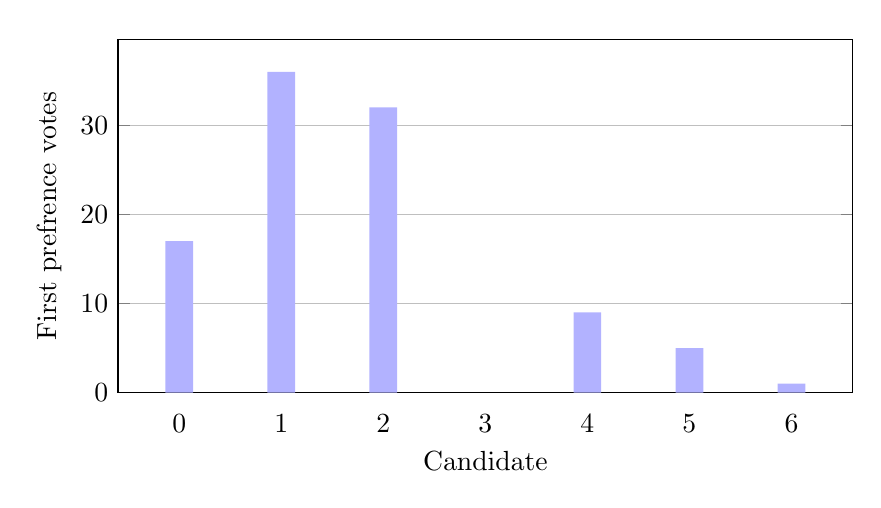
\begin{tikzpicture}
		\begin{axis}[
			ybar,
			width = 0.9\textwidth,
			height = 0.5\textwidth,
			legend style={at={(0.5,-0.25)},
			anchor=north,legend columns=-1},
      x tick style = transparent,
			ylabel = {First prefrence votes},
			xlabel = {Candidate},
			ymajorgrids = true,
			every axis plot/.append style={fill,draw=none,no markers},
      ymin = 0
      ]
			\addplot coordinates
			{(0, 17)(1, 36)(2, 32)(4, 9)(5, 5)(6, 1)};
		\end{axis}
	\end{tikzpicture}
\end{figure}



\printbibliography


\section{Appendix}
First-past-the-post program


\end{document}
